\lettrine[lhang=0.17]{W}{e've seen two basic} ways of combining types: using a product and a
coproduct. It turns out that a lot of data structures in everyday
programming can be built using just these two mechanisms. This fact has
important practical consequences. Many properties of data structures are
composable. For instance, if you know how to compare values of basic
types for equality, and you know how to generalize these comparisons to
product and coproduct types, you can automate the derivation of equality
operators for composite types. In Haskell you can automatically derive
equality, comparison, conversion to and from string, and more, for a
large subset of composite types.

Let's have a closer look at product and sum types as they appear in
programming.

\section{Product Types}\label{product-types}

The canonical implementation of a product of two types in a programming
language is a pair. In Haskell, a pair is a primitive type constructor;
in C++ it's a relatively complex template defined in the Standard
Library.

\begin{figure}
  \centering
  \fbox{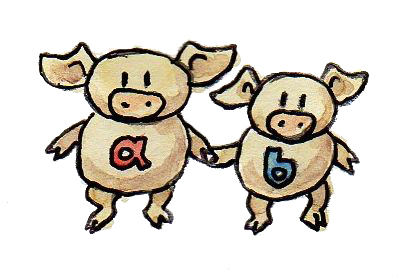
\includegraphics[width=1.56250in]{images/pair.jpg}}
\end{figure}

\noindent
Pairs are not strictly commutative: a pair \code{(Int,\ Bool)} cannot
be substituted for a pair \code{(Bool,\ Int)}, even though they carry
the same information. They are, however, commutative up to isomorphism
--- the isomorphism being given by the \code{swap} function (which is
its own inverse):

\begin{verbatim}
swap :: (a, b) -> (b, a)
swap (x, y) = (y, x)
\end{verbatim}

\noindent
You can think of the two pairs as simply using a different format for
storing the same data. It's just like big endian vs. little endian.

You can combine an arbitrary number of types into a product by nesting
pairs inside pairs, but there is an easier way: nested pairs are
equivalent to tuples. It's the consequence of the fact that different
ways of nesting pairs are isomorphic. If you want to combine three types
in a product, \code{a}, \code{b}, and \code{c}, in this order, you
can do it in two ways:

\begin{verbatim}
((a, b), c)
\end{verbatim}

\noindent
or

\begin{verbatim}
(a, (b, c))
\end{verbatim}

\noindent
These types are different --- you can't pass one to a function that
expects the other --- but their elements are in one-to-one
correspondence. There is a function that maps one to another:

\begin{verbatim}
alpha :: ((a, b), c) -> (a, (b, c))
alpha ((x, y), z) = (x, (y, z))
\end{verbatim}

\noindent
and this function is invertible:

\begin{verbatim}
alpha_inv :: (a, (b, c)) -> ((a, b), c)
alpha_inv (x, (y, z)) = ((x, y), z)
\end{verbatim}

\noindent
so it's an isomorphism. These are just different ways of repackaging the
same data.

You can interpret the creation of a product type as a binary operation
on types. From that perspective, the above isomorphism looks very much
like the associativity law we've seen in monoids:

\begin{verbatim}
(a * b) * c = a * (b * c)
\end{verbatim}

Except that, in the monoid case, the two ways of composing products were
equal, whereas here they are only equal ``up to isomorphism.''

If we can live with isomorphisms, and don't insist on strict equality,
we can go even further and show that the unit type, \code{()}, is the
unit of the product the same way 1 is the unit of multiplication.
Indeed, the pairing of a value of some type \code{a} with a unit
doesn't add any information. The type:

\begin{verbatim}
(a, ())
\end{verbatim}

\noindent
is isomorphic to \code{a}. Here's the isomorphism:

\begin{verbatim}
rho :: (a, ()) -> a
rho (x, ()) = x
\end{verbatim}

\begin{verbatim}
rho_inv :: a -> (a, ())
rho_inv x = (x, ())
\end{verbatim}

\noindent
These observations can be formalized by saying that \textbf{Set} (the
category of sets) is a \newterm{monoidal category}. It's a category that's
also a monoid, in the sense that you can multiply objects (here, take
their cartesian product). I'll talk more about monoidal categories, and
give the full definition in the future.

There is a more general way of defining product types in Haskell ---
especially, as we'll see soon, when they are combined with sum types. It
uses named constructors with multiple arguments. A pair, for instance,
can be defined alternatively as:

\begin{verbatim}
data Pair a b = P a b
\end{verbatim}

Here, \code{Pair\ a\ b} is the name of the type paremeterized by two
other types, \code{a} and \code{b}; and \code{P} is the name of
the data constructor. You define a pair type by passing two types to the
\code{Pair} type constructor. You construct a pair value by passing
two values of appropriate types to the constructor \code{P}. For
instance, let's define a value \code{stmt} as a pair of
\code{String} and \code{Bool}:

\begin{verbatim}
stmt :: Pair String Bool
stmt = P "This statements is" False
\end{verbatim}

\noindent
The first line is the type declaration. It uses the type constructor
\code{Pair}, with \code{String} and \code{Bool} replacing
\code{a} and the \code{b} in the generic definition of
\code{Pair}. The second line defines the actual value by passing a
concrete string and a concrete Boolean to the data constructor
\code{P}. Type constructors are used to construct types; data
constructors, to construct values.

Since the name spaces for type and data constructors are separate in
Haskell, you will often see the same name used for both, as in:

\begin{verbatim}
data Pair a b = Pair a b
\end{verbatim}

\noindent
And if you squint hard enough, you may even view the built-in pair type
as a variation on this kind of declaration, where the name \code{Pair}
is replaced with the binary operator \code{(,)}. In fact you can use
\code{(,)} just like any other named constructor and create pairs
using prefix notation:

\begin{verbatim}
stmt = (,) "This statement is" False
\end{verbatim}

\noindent
Similarly, you can use \code{(,,)} to create triples, and so on.

Instead of using generic pairs or tuples, you can also define specific
named product types, as in:

\begin{verbatim}
data Stmt = Stmt String Bool
\end{verbatim}

\noindent
which is just a product of \code{String} and \code{Bool}, but it's
given its own name and constructor. The advantage of this style of
declaration is that you may define many types that have the same content
but different meaning and functionality, and which cannot be substituted
for each other.

Programming with tuples and multi-argument constructors can get messy
and error prone --- keeping track of which component represents what.
It's often preferable to give names to components. A product type with
named fields is called a record in Haskell, and a \code{struct} in C.

\section{Records}\label{records}

Let's have a look at a simple example. We want to describe chemical
elements by combining two strings, name and symbol; and an integer, the
atomic number; into one data structure. We can use a tuple
\code{(String,\ String,\ Int)} and remember which component represents
what. We would extract components by pattern matching, as in this
function that checks if the symbol of the element is the prefix of its
name (as in \textbf{He} being the prefix of \textbf{Helium}):

\begin{verbatim}
startsWithSymbol :: (String, String, Int) -> Bool
startsWithSymbol (name, symbol, _) = isPrefixOf symbol name
\end{verbatim}

\noindent
This code is error prone, and is hard to read and maintain. It's much
better to define a record:

\begin{verbatim}
data Element = Element { name :: String 
                       , symbol :: String 
                       , atomicNumber :: Int }
\end{verbatim}

\noindent
The two representations are isomorphic, as witnessed by these two
conversion functions, which are the inverse of each other:

\begin{verbatim}
tupleToElem :: (String, String, Int) -> Element
tupleToElem (n, s, a) = Element { name = n 
                                , symbol = s 
                                , atomicNumber = a }
\end{verbatim}

\begin{verbatim}
elemToTuple :: Element -> (String, String, Int)
elemToTuple e = (name e, symbol e, atomicNumber e)
\end{verbatim}

\noindent
Notice that the names of record fields also serve as functions to access
these fields. For instance, \code{atomicNumber e} retrieves the
\code{atomicNumber} field from \code{e}. We use
\code{atomicNumber} as a function of the type:

\begin{verbatim}
atomicNumber :: Element -> Int
\end{verbatim}

With the record syntax for \code{Element}, our function
\code{startsWithSymbol} becomes more readable:

\begin{verbatim}
startsWithSymbol :: Element -> Bool
startsWithSymbol e = isPrefixOf (symbol e) (name e)
\end{verbatim}

\noindent
We could even use the Haskell trick of turning the function
\code{isPrefixOf} into an infix operator by surrounding it with
backquotes, and make it read almost like a sentence:

\begin{verbatim}
startsWithSymbol e = symbol e `isPrefixOf` name e
\end{verbatim}

\noindent
The parentheses could be omitted in this case, because an infix operator
has lower precedence than a function call.

\section{Sum Types}\label{sum-types}

Just as the product in the category of sets gives rise to product types,
the coproduct gives rise to sum types. The canonical implementation of a
sum type in Haskell is:

\begin{verbatim}
data Either a b = Left a | Right b
\end{verbatim}

\noindent
And like pairs, \code{Either}s are commutative (up to isomorphism),
can be nested, and the nesting order is irrelevant (up to isomorphism).
So we can, for instance, define a sum equivalent of a triple:

\begin{verbatim}
data OneOfThree a b c = Sinistral a | Medial b | Dextral c
\end{verbatim}

\noindent
and so on.

It turns out that \textbf{Set} is also a (symmetric) monoidal category
with respect to coproduct. The role of the binary operation is played by
the disjoint sum, and the role of the unit element is played by the
initial object. In terms of types, we have \code{Either} as the
monoidal operator and \code{Void}, the uninhabited type, as its
neutral element. You can think of \code{Either} as plus, and
\code{Void} as zero. Indeed, adding \code{Void} to a sum type
doesn't change its content. For instance:

\begin{verbatim}
Either a Void
\end{verbatim}

\noindent
is isomorphic to \code{a}. That's because there is no way to construct
a \code{Right} version of this type --- there isn't a value of type
\code{Void}. The only inhabitants of \code{Either\ a\ Void} are
constructed using the \code{Left} constructors and they simply
encapsulate a value of type \code{a}. So, symbolically,
\code{a\ +\ 0\ =\ a}.

Sum types are pretty common in Haskell, but their C++ equivalents,
unions or variants, are much less common. There are several reasons for
that.

First of all, the simplest sum types are just enumerations and are
implemented using \code{enum} in C++. The equivalent of the Haskell
sum type:

\begin{verbatim}
data Color = Red | Green | Blue
\end{verbatim}

\noindent
is the C++:

\begin{verbatim}
enum { Red, Green, Blue };
\end{verbatim}

\noindent
An even simpler sum type:

\begin{verbatim}
data Bool = True | False
\end{verbatim}

\noindent
is the primitive \code{bool} in C++.

Simple sum types that encode the presence or absence of a value are
variously implemented in C++ using special tricks and ``impossible''
values, like empty strings, negative numbers, null pointers, etc. This
kind of optionality, if deliberate, is expressed in Haskell using the
\code{Maybe} type:

\begin{verbatim}
data Maybe a = Nothing | Just a
\end{verbatim}

\noindent
The \code{Maybe} type is a sum of two types. You can see this if you
separate the two constructors into individual types. The first one would
look like this:

\begin{verbatim}
data NothingType = Nothing
\end{verbatim}

\noindent
It's an enumeration with one value called \code{Nothing}. In other
words, it's a singleton, which is equivalent to the unit type
\code{()}. The second part:

\begin{verbatim}
data JustType a = Just a
\end{verbatim}

\noindent
is just an encapsulation of the type \code{a}. We could have encoded
\code{Maybe} as:

\begin{verbatim}
data Maybe a = Either () a
\end{verbatim}

\noindent
More complex sum types are often faked in C++ using pointers. A pointer
can be either null, or point to a value of specific type. For instance,
a Haskell list type, which can be defined as a (recursive) sum type:

\begin{verbatim}
List a = Nil | Cons a (List a)
\end{verbatim}

\noindent
can be translated to C++ using the null pointer trick to implement the
empty list:

\begin{verbatim}
template<class A>
class List { 
    Node<A> * _head;
public:
    List() : _head(nullptr) {} // Nil
    List(A a, List<A> l)       // Cons
      : _head(new Node<A>(a, l))
    {}
};
\end{verbatim}

\noindent
Notice that the two Haskell constructors \code{Nil} and \code{Cons}
are translated into two overloaded \code{List} constructors with
analogous arguments (none, for \code{Nil}; and a value and a list for
\code{Cons}). The \code{List} class doesn't need a tag to
distinguish between the two components of the sum type. Instead it uses
the special \code{nullptr} value for \code{\_head} to encode
\code{Nil}.

The main difference, though, between Haskell and C++ types is that
Haskell data structures are immutable. If you create an object using one
particular constructor, the object will forever remember which
constructor was used and what arguments were passed to it. So a
\code{Maybe} object that was created as \code{Just "energy"} will
never turn into \code{Nothing}. Similarly, an empty list will forever
be empty, and a list of three elements will always have the same three
elements.

It's this immutability that makes construction reversible. Given an
object, you can always disassemble it down to parts that were used in
its construction. This deconstruction is done with pattern matching and
it reuses constructors as patterns. Constructor arguments, if any, are
replaced with variables (or other patterns).

The \code{List} data type has two constructors, so the deconstruction
of an arbitrary \code{List} uses two patterns corresponding to those
constructors. One matches the empty \code{Nil} list, and the other a
\code{Cons}-constructed list. For instance, here's the definition of a
simple function on \code{List}s:

\begin{verbatim}
maybeTail :: List a -> Maybe (List a)
maybeTail Nil = Nothing
maybeTail (Cons _ t) = Just t
\end{verbatim}

\noindent
The first part of the definition of \code{maybeTail} uses the
\code{Nil} constructor as pattern and returns \code{Nothing}. The
second part uses the \code{Cons} constructor as pattern. It replaces
the first constructor argument with a wildcard, because we are not
interested in it. The second argument to \code{Cons} is bound to the
variable \code{t} (I will call these things variables even though,
strictly speaking, they never vary: once bound to an expression, a
variable never changes). The return value is \code{Just\ t}. Now,
depending on how your \code{List} was created, it will match one of
the clauses. If it was created using \code{Cons}, the two arguments
that were passed to it will be retrieved (and the first discarded).

Even more elaborate sum types are implemented in C++ using polymorphic
class hierarchies. A family of classes with a common ancestor may be
understood as one variant type, in which the vtable serves as a hidden
tag. What in Haskell would be done by pattern matching on the
constructor, and by calling specialized code, in C++ is accomplished by
dispatching a call to a virtual function based on the vtable pointer.

You will rarely see \code{union} used as a sum type in C++ because of
severe limitations on what can go into a union. You can't even put a
\code{std::string} into a union because it has a copy constructor.

\section{Algebra of Types}\label{algebra-of-types}

Taken separately, product and sum types can be used to define a variety
of useful data structures, but the real strength comes from combining
the two. Once again we are invoking the power of composition.

Let's summarize what we've discovered so far. We've seen two commutative
monoidal structures underlying the type system: We have the sum types
with \code{Void} as the neutral element, and the product types with
the unit type, \code{()}, as the neutral element. We'd like to think
of them as analogous to addition and multiplication. In this analogy,
\code{Void} would correspond to zero, and unit, \code{()}, to one.

Let's see how far we can stretch this analogy. For instance, does
multiplication by zero give zero? In other words, is a product type with
one component being \code{Void} isomorphic to \code{Void}? For
example, is it possible to create a pair of, say \code{Int} and
\code{Void}?

To create a pair you need two values. Although you can easily come up
with an integer, there is no value of type \code{Void}. Therefore, for
any type \code{a}, the type \code{(a,\ Void)} is uninhabited --- has
no values --- and is therefore equivalent to \code{Void}. In other
words, \code{a*0 = 0}.

Another thing that links addition and multiplication is the distributive
property:

\begin{verbatim}
a * (b + c) = a * b + a * c
\end{verbatim}

\noindent
Does it also hold for product and sum types? Yes, it does --- up to
isomorphisms, as usual. The left hand side corresponds to the type:

\begin{verbatim}
(a, Either b c)
\end{verbatim}

\noindent
and the right hand side corresponds to the type:

\begin{verbatim}
Either (a, b) (a, c)
\end{verbatim}

\noindent
Here's the function that converts them one way:

\begin{verbatim}
prodToSum :: (a, Either b c) -> Either (a, b) (a, c)
prodToSum (x, e) = 
    case e of
      Left  y -> Left  (x, y)
      Right z -> Right (x, z)
\end{verbatim}

\noindent
and here's one that goes the other way:

\begin{verbatim}
sumToProd :: Either (a, b) (a, c) -> (a, Either b c)
sumToProd e =
    case e of
      Left  (x, y) -> (x, Left  y)
      Right (x, z) -> (x, Right z)
\end{verbatim}

\noindent
The \code{case\ of} statement is used for pattern matching inside
functions. Each pattern is followed by an arrow and the expression to be
evaluated when the pattern matches. For instance, if you call
\code{prodToSum} with the value:

\begin{verbatim}
prod1 :: (Int, Either String Float)
prod1 = (2, Left "Hi!")
\end{verbatim}

\noindent
the \code{e} in \code{case e of} will be equal to
\code{Left "Hi!"}. It will match the pattern \code{Left y},
substituting \code{"Hi!"} for \code{y}. Since the \code{x} has
already been matched to \code{2}, the result of the \code{case of}
clause, and the whole function, will be \code{Left (2, "Hi!")}, as
expected.

I'm not going to prove that these two functions are the inverse of each
other, but if you think about it, they must be! They are just trivially
re-packing the contents of the two data structures. It's the same data,
only different format.

Mathematicians have a name for such two intertwined monoids: it's called
a \newterm{semiring}. It's not a full \newterm{ring}, because we can't define
subtraction of types. That's why a semiring is sometimes called a
\newterm{rig}, which is a pun on ``ring without an \emph{n}'' (negative).
But barring that, we can get a lot of mileage from translating
statements about, say, natural numbers, which form a rig, to statements
about types. Here's a translation table with some entries of interest:

\begin{longtable}[]{@{}ll@{}}
\toprule
Numbers & Types\tabularnewline
\midrule
\endhead
0 & \code{Void}\tabularnewline
1 & \code{()}\tabularnewline
a + b &
\code{Either a b = Left a | Right b}\tabularnewline
a * b & \code{(a, b)} or 
\code{Pair a b = Pair a b}\tabularnewline
2 = 1 + 1 &
\code{data Bool = True | False}\tabularnewline
1 + a &
\code{data Maybe = Nothing | Just a}\tabularnewline
\bottomrule
\end{longtable}

\noindent
The list type is quite interesting, because it's defined as a solution
to an equation. The type we are defining appears on both sides of the
equation:

\begin{verbatim}
List a = Nil | Cons a (List a)
\end{verbatim}

\noindent
If we do our usual substitutions, and also replace \code{List\ a} with
\code{x}, we get the equation:

\begin{verbatim}
x = 1 + a * x
\end{verbatim}

\noindent
We can't solve it using traditional algebraic methods because we can't
subtract or divide types. But we can try a series of substitutions,
where we keep replacing \code{x} on the right hand side with
\code{(1 + a*x)}, and use the distributive property. This leads to
the following series:

\begin{verbatim}
x = 1 + a*x
x = 1 + a*(1 + a*x) = 1 + a + a*a*x
x = 1 + a + a*a*(1 + a*x) = 1 + a + a*a + a*a*a*x
...
x = 1 + a + a*a + a*a*a + a*a*a*a...
\end{verbatim}

\noindent
We end up with an infinite sum of products (tuples), which can be
interpreted as: A list is either empty, \code{1}; or a singleton,
\code{a}; or a pair, \code{a*a}; or a triple, \code{a*a*a};
etc\ldots{} Well, that's exactly what a list is --- a string of
\code{a}s!

There's much more to lists than that, and we'll come back to them and
other recursive data structures after we learn about functors and fixed
points.

Solving equations with symbolic variables --- that's algebra! It's what
gives these types their name: algebraic data types.

Finally, I should mention one very important interpretation of the
algebra of types. Notice that a product of two types \code{a} and
\code{b} must contain both a value of type \code{a} \emph{and} a
value of type \code{b}, which means both types must be inhabited. A
sum of two types, on the other hand, contains either a value of type
\code{a} \emph{or} a value of type \code{b}, so it's enough if one
of them is inhabited. Logical \emph{and} and \emph{or} also form a
semiring, and it too can be mapped into type theory:

\begin{longtable}[]{@{}ll@{}}
\toprule
Logic & Types\tabularnewline
\midrule
\endhead
false & \code{Void}\tabularnewline
true & \code{()}\tabularnewline
a \textbar{}\textbar{} b &
\code{Either a b = Left a | Right b}\tabularnewline
a \&\& b & \code{(a, b)}\tabularnewline
\bottomrule
\end{longtable}

\noindent
This analogy goes deeper, and is the basis of the Curry-Howard
isomorphism between logic and type theory. We'll come back to it when we
talk about function types.

\section{Challenges}\label{challenges}

\begin{enumerate}
\tightlist
\item
  Show the isomorphism between \code{Maybe a} and
  \code{Either () a}.
\item
  Here's a sum type defined in Haskell:

\begin{verbatim}
data Shape = Circle Float 
           | Rect Float Float
\end{verbatim}

  When we want to define a function like \code{area} that acts on a
  \code{Shape}, we do it by pattern matching on the two constructors:

\begin{verbatim}
area :: Shape -> Float
area (Circle r) = pi * r * r
area (Rect d h) = d * h
\end{verbatim}

  Implement \code{Shape} in C++ or Java as an interface and create two
  classes: \code{Circle} and \code{Rect}. Implement \code{area} as
  a virtual function.
\item
  Continuing with the previous example: We can easily add a new function
  \code{circ} that calculates the circumference of a \code{Shape}.
  We can do it without touching the definition of \code{Shape}:

\begin{verbatim}
circ :: Shape -> Float
circ (Circle r) = 2.0 * pi * r
circ (Rect d h) = 2.0 * (d + h)
\end{verbatim}

  Add \code{circ} to your C++ or Java implementation. What parts of
  the original code did you have to touch?
\item
  Continuing further: Add a new shape, \code{Square}, to
  \code{Shape} and make all the necessary updates. What code did you
  have to touch in Haskell vs. C++ or Java? (Even if you're not a
  Haskell programmer, the modifications should be pretty obvious.)
\item
  Show that \code{a\ +\ a\ =\ 2\ *\ a} holds for types (up to
  isomorphism). Remember that \code{2} corresponds to \code{Bool},
  according to our translation table.
\end{enumerate}

\section{Acknowledments}\label{acknowledments}

Thanks go to Gershom Bazerman for reviewing this post and helpful
comments.
